\chapter{Анализ существующих решений}

У каждого из типов рекомендательных систем, которые были разобраны в анализе предметной области, 
существует большое количество различных вариаций методов и алгоритмов, реализующих эти подходы.
В данном разделе будут рассмотрены наиболее популярные и широко применимые методы. 

\section{Коллаборативная фильтрация}

Основная идея методов коллаборативных рекомендаций заключается в использовании данных о прошлом поведении или
мнениях существующего сообщества пользователей для предсказания, какие товары могут понравиться текущему пользователю.
Такие системы широко применяются в индустрии, особенно на онлайн-ретейл-платформах, где они помогают адаптировать
контент под конкретного клиента, способствуя увеличению продаж и продвижению дополнительных товаров.
На данный момент есть два базовых пути проектирования рекомендательных систем на основе коллаборативной фильтрации:
кластеризация объектов на основе оценок других пользователей (user - based) и предметов
(item - based)~\cite{rek_intro}.

\subsection*{User-based метод}
При использовании user-based подхода основная идея состоит в поиске пользователей, чьи предпочтения близки к предпочтениям рассматриваемого пользователя.
Для этого вычисляется мера сходства между пользователями на основе их оценок одних и тех же объектов.
Часто применяются такие метрики, как корреляция Пирсона или нормированный косинусный коэффициент,
учитывающие средние значения рейтингов, что позволяет компенсировать различия в «шкале» оценок различных пользователей.
После нахождения близких по предпочтениям пользователей предсказание рейтинга для конкретного объекта осуществляется как
средневзвешенное отклонение их оценок от собственных средних оценок.
Например, предсказанный рейтинг для пользователя \(u\) и объекта \(i\) может быть выражен формулой:

\begin{equation}
	\hat{R}_{u,i} = \bar{R}_u + \frac{\sum_{v \in U_i} \text{sim}(u,v)(R_{v,i}-\bar{R}_v)}{\sum_{v \in U_i} \text{sim}(u,v)},
\end{equation}

где \(\bar{R}_u\) — средний рейтинг пользователя \(u\), \(R_{v,i}\) — рейтинг пользователя \(v\) для объекта \(i\),
а \(\text{sim}(u,v)\) — степень сходства между пользователями \(u\) и \(v\). Множество \(U_i\) состоит из пользователей,
оценивших объект \(i\)~\cite{col_rek}.

\subsection*{Item-based метод}

Item-based подход базируется на определении сходства между самими объектами, а не между пользователями.
Предполагается, что объекты, получающие сходные оценки от множества пользователей, вероятно, имеют схожие характеристики.
При этом можно использовать те же метрики, что и в user-based подходе, например, корреляцию Пирсона или нормированный
косинус, но теперь применительно к вектору оценок объектов. После определения степени сходства между объектами
предсказание рейтинга для пользователя \(u\) и ещё не оцененного им объекта \(i\) основывается на оценках,
которые этот пользователь уже поставил похожим объектам, с учётом весового вклада их сходства с объектом \(i\):

\begin{equation}
\hat{R}_{u,i} = \bar{R}_u + \frac{\sum_{j \in I_u} \text{sim}(i,j)(R_{u,j}-\bar{R}_u)}{\sum_{j \in I_u} \text{sim}(i,j)},
\end{equation}

где \(\bar{R}_u\) — средний рейтинг пользователя \(u\), \(R_{u,j}\) — рейтинг пользователя \(u\) для объекта \(j\),
\(\text{sim}(i,j)\) — мера сходства между объектами \(i\) и \(j\), а \(I_u\) — множество объектов, оцененных пользователем
\(u\)~\cite{col_rek}.

\section{Контентно-ориентированные методы}

Системы, использующие подход рекомендаций на основе контента, анализируют описания объектов,
ранее оцененных пользователем, и создают профиль его интересов на основе характеристик этих объектов.
Этот профиль используется для рекомендации новых элементов, представляющих интерес.
Процесс рекомендации заключается в сопоставлении атрибутов профиля пользователя с атрибутами контентного объекта,
что позволяет оценить его релевантность для пользователя.
Точный профиль значительно повышает эффективность доступа к информации, например,
фильтруя результаты поиска и скрывая страницы, которые не интересуют пользователя~\cite{def_rec}.

Системы фильтрации информации, основанные на содержании, нуждаются в подходящих методах
для представления объектов и формирования профиля пользователя, а также в стратегиях для сравнения профиля
пользователя с представлением объектов.
Высокоуровневая архитектура рекомендательной системы,
основанной на содержании, изображена на рисунке~\ref{img:rtp_udp}.

\begin{figure}[h]
	\centering
	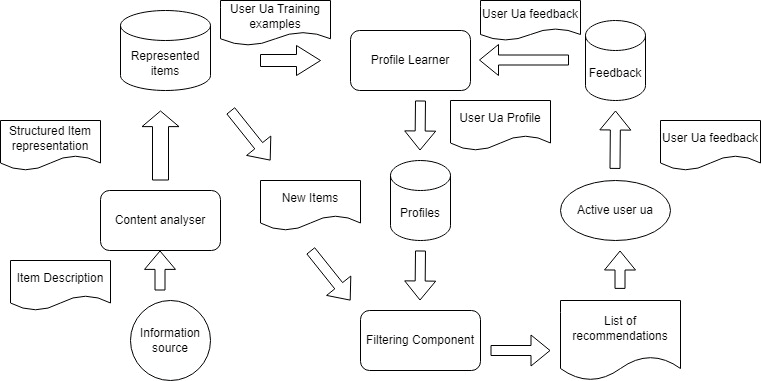
\includegraphics[width=0.8\textwidth]{images/contrek}
	\caption{Высокоуровневая архитектура рекомендательной системы, основанной на содержании~\cite{def_rec}}
	\label{img:rtp_udp}
\end{figure}

Процесс рекомендации выполняется в три этапа, каждый из которых
обрабатывается отдельным компонентом.

\subsection*{Анализатор содержания (Content analyser)}
Когда информация не имеет структуры (например, текст), требуется предварительная
обработка для извлечения структурированной релевантной информации.
Основная задача компонента – представлять содержание объектов (например, документов, веб-страниц,
новостей, описаний продуктов и т. д.), поступающих из источников информации, в форме,
подходящей для последующей обработки~\cite{def_rec}.

\subsection*{Обучение профиля (Profile Learner)}
Этот модуль собирает данные, отражающие предпочтения пользователя, и пытается обобщить их
для создания профиля пользователя.
Обычно стратегия обобщения реализуется с помощью методов машинного обучения,
способных создать модель интересов пользователя, основываясь на объектах, которые ему нравились или
не нравились ранее~\cite{def_rec}.

\subsection*{Компонент фильтрации (Filtering component)}
Этот модуль использует профиль пользователя для предложения релевантных объектов,
сопоставляя представление профиля с представлением объектов для рекомендации.
Результат может быть в виде бинарного или непрерывного определения релевантности, причем в последнем случае это список
потенциально интересных объектов, упорядоченный по убыванию релевантности~\cite{def_rec}.

\section{Методы, основанные на знаниях}

Рекомендации, основанные на знаниях, используются обычно в таких
областях, как электроника, где покупатели совершают покупки раз в
пару лет, так как в данной области мы не можем положиться на историю
покупок, которая используется в качестве входных данных для методов
коллаборативной фильтрации и методов, основанных на содержании.\cite{kut_rec}

Системы, которые опираются на источники знаний, не используемые в коллаборативных и контентных подходах,
по определению считаются системами, основанными на знаниях.
Существует два основных типа рекомендательных систем, основанных на знаниях~\cite{rek_intro}:

\begin{itemize}
\item системы, основанные на ограничениях (constraint-based);
\item системы, основанные на примерах (case-based).
\end{itemize}

\subsection*{Системы, основанные на ограничениях (constraint-based)}

Классическая задача удовлетворения ограничений (CSP) может быть описана кортежем \((V, D, C)\), где:
\begin{itemize}
    \item \(V\) – множество переменных;
    \item \(D\) – множество конечных доменов для этих переменных;
    \item \(C\) – множество ограничений, описывающих комбинации значений, которые переменные могут одновременно принимать.
\end{itemize}

Решение CSP соответствует присвоению значения каждой переменной из \(V\) таким образом, чтобы все ограничения были выполнены~\cite{rek_intro}.

Рекомендательные системы, основанные на ограничениях, могут использовать эту формализацию,
применяя базу знаний рекомендаций, которая обычно включает два различных набора переменных $V = V_C \cup V_{PROD}$.
\(V_C\) описывает потенциальные требования клиента, например, максимальная цена, приемлемая для клиента.
\(V_{PROD}\) описывает свойства продуктов, например, возможное разрешение цифровой камеры~\cite{rek_intro}.

Три различных набора ограничений $C = C_R \cup C_F \cup C_{PROD}$ определяют, какие товары следует рекомендовать
клиенту в определенной ситуации~\cite{rek_intro}.

\begin{enumerate}
    \item Ограничения совместимости (\(C_R\)) определяют допустимые значения свойств клиента. Например, если требуются фотографии для печати большого размера, максимальная допустимая цена должна быть выше 200.
    \item Условия фильтрации (\(C_F\)) определяют, при каких условиях должны быть выбраны определенные товары. Например, фотографии большого размера требуют разрешения более 5 мегапикселей.
    \item Ограничения продуктов (\(C_{PROD}\)) определяют текущий доступный ассортимент продуктов. Каждая конъюнкция в этом ограничении полностью описывает продукт (товар) – все свойства продукта имеют заданное значение.
\end{enumerate}

\subsection*{Системы, основанные на примерах (constraint-based)}

В подходах рекомендаций на основе случаев элементы выбираются с использованием мер схожести,
которые описывают, насколько свойства элементов соответствуют заданным требованиям пользователя.
Так называемая дистанционная схожесть элемента \(i\) с требованиями \(r \in REQ\) часто определяется,
как показано в формуле~\ref{eq:sim1}.

В данном контексте \(sim(i, r)\) выражает для каждого значения атрибута элемента \(\varphi_r(i)\) его
расстояние до требования пользователя \(r \in REQ\).
Кроме того, \(w_r\) представляет собой вес важности для требования \(r\)~\cite{rek_intro}.

\begin{equation}
\text{similarity}(i, REQ) = \frac{\sum_{r \in REQ} w_r \cdot \text{sim}(i, r)}{\sum_{r \in REQ} w_r}
\label{eq:sim1}
\end{equation}

%В реальных сценариях есть свойства, которые клиент хотел бы максимизировать, например, разрешение цифровой камеры.
%Также существуют свойства, которые клиент хотел бы минимизировать, например, цену цифровой камеры или уровень риска
%финансовой услуги. В первом случае речь идет о свойствах <<больше — лучше>> (MIB, More-Is-Better), а во втором — о
%свойствах <<меньше — лучше>>(LIB, Less-Is-Better).~\cite{rek_intro}
%
%Чтобы учитывать эти базовые свойства в наших расчетах схожести, мы вводим следующие формулы для
%расчета локальной схожести. Во-первых, в случае свойств MIB локальная схожесть между \(i\) и \(r\) рассчитывается
%следующим образом:
%
%\begin{equation}
%\text{sim}(i, r) = \frac{\varphi_r(i) - \min(r)}{\max(r) - \min(r)}
%\end{equation}
%
%Локальная схожесть между \(i\) и \(r\) в случае свойств LIB рассчитывается следующим образом:
%
%\begin{equation}
%\text{sim}(i, r) = \frac{\max(r) - \varphi_r(i)}{\max(r) - \min(r)}
%\end{equation}
%
%Наконец, есть ситуации, в которых схожесть должна основываться исключительно на расстоянии до изначально заданных требований.
%Например, если пользователь указал желаемое время выполнения финансовой услуги или размер монитора,
%минимальное время выполнения или самый большой монитор не будут представлять оптимальное решение.
%Для таких случаев мы вводим третий тип локальной функции схожести:
%
%\begin{equation}
%\text{sim}(i, r) = 1 - \frac{|\varphi_r(i) - r|}{\max(r) - \min(r)}
%\end{equation}
%
%Рассмотренные в данном разделе меры схожести часто служат основой для различных систем рекомендаций на основе случаев.~\cite{rek_intro}

\section{Гибридные системы}

Каждый из вышеописанных методов имеет свои преимущества и недостатки в
зависимости от поставленной задачи. Достаточно очевидным
решением всех этих проблем является объединение различных подходов
для того, чтобы обеспечить большую точность рекомендаций~\cite{kut_rec}.

Если, например, у нас есть данные об описании продуктов, профиль
пользователей и история его покупок, то мы можем улучшить рекомендательную
систему путем объединения методов коллаборативной фильтрации
и алгоритмов фильтрации по содержанию. Таким образом, в случае появления
нового пользователя в системе, о котором нет истории
покупок, мы сможем использовать рекомендации на основе алгоритмов
фильтрации по содержанию, а в случае большого объема статистических
данных строить более точный прогноз, используя методы коллаборативной фильтрации~\cite{kut_rec}.

Различные способы объединения коллаборативных и контентных методов в
гибридной рекомендательной системе можно классифицировать следующим образом~\cite{hist}.

\begin{enumerate}
\item Раздельная реализация коллаборативного и контентного методов с последующим объединением их предсказаний.
\item Включение некоторых характеристик контентного подхода в коллаборативный метод и наоборот.
%\item Включение некоторых характеристик коллаборативного подхода в контентный метод.
\item Построение общей унифицированной модели, которая включает как контентные, так и коллаборативные характеристики.
\end{enumerate}



